\chapter{High-Level Design}
\label{ch:hld}

\section{Design Goals}

\begin{itemize}
\item \textbf{Tooth-centric output.} The unit of every result is a numbered tooth, because that is
  how a dentist reads and records an OPG.
\item \textbf{One code path.} The command-line tool and the web demo call the same two functions
  (\texttt{load\_models}, \texttt{run\_pipeline}), so a fix or a new caveat reaches both and the demo
  cannot drift from what the evaluation measured.
\item \textbf{Modular stages.} Each stage is trained on the dataset that carries its label and can
  be replaced by another checkpoint without touching the others.
\item \textbf{Honest output.} The report carries the measured limitations of whichever checkpoints
  ran, next to the findings.
\item \textbf{Commodity hardware.} Inference on a CPU, packaged in a container.
\end{itemize}

\section{System Architecture}

The system is organised in five layers (Figure~\ref{fig:layers}). The presentation layer holds the
two entry points. The orchestration layer loads the models once, checks the input, runs the stages
in order and records provenance. The stage layer contains the six pipeline stages. The model and
artefact layer holds the hash-pinned checkpoints and the outputs. Beside them, an evaluation layer of
scripts and tests reproduces every number reported in Chapter~\ref{ch:results}.

\begin{figure}[!htbp]
\centering
% Layered architecture. Components traced to: app.py, scripts/run_inference.py (main, load_models,
% run_pipeline, runtime_info, check_input, build_report, draw_overlay), src/*.py, models/README.md,
% scripts/eval/, scripts/verify_paper_numbers.py, tests/.
\begin{tikzpicture}[
  lay/.style={rectangle,rounded corners=3pt,draw=#1,line width=0.8pt,fill=#1!6,minimum width=128mm,
              minimum height=14mm,inner sep=3pt},
  lname/.style={font=\sffamily\scriptsize\bfseries,text=#1,anchor=west},
  comp/.style={box,fill=#1,text width=27mm,minimum height=8mm,font=\sffamily\tiny\bfseries}]
% layers
\node[lay=p2grey]   (L1) at (0,0)     {};
\node[lay=p2indigo] (L2) at (0,-1.75) {};
\node[lay=p2teal,minimum height=17mm] (L3) at (0,-3.85) {};
\node[lay=p2green]  (L4) at (0,-5.75) {};
\node[lname=p2grey]   at ($(L1.north west)+(1mm,-2mm)$) {Presentation};
\node[lname=p2indigo] at ($(L2.north west)+(1mm,-2mm)$) {Orchestration};
\node[lname=p2teal]   at ($(L3.north west)+(1mm,-2mm)$) {Stages};
\node[lname=p2green]  at ($(L4.north west)+(1mm,-2mm)$) {Models and artefacts};
% presentation
\node[comp=p2grey] at (-2.2,-0.15) {CLI\\\texttt{run\_inference.py main}};
\node[comp=p2grey] at (2.2,-0.15)  {Web demo\\\texttt{app.py} (Streamlit)};
% orchestration
\node[comp=p2indigo] at (-4.4,-1.9) {\texttt{load\_models}\\hash-pinned loads};
\node[comp=p2indigo] at (-1.45,-1.9) {\texttt{check\_input}\\input warnings};
\node[comp=p2indigo] at (1.5,-1.9)  {\texttt{run\_pipeline}\\Stages 1--6};
\node[comp=p2indigo] at (4.45,-1.9) {\texttt{runtime\_info}\\provenance};
% stages (two rows)
\node[comp=p2teal,text width=19mm] at (-5.05,-4.0) {1 Detect\\YOLOv11l};
\node[comp=p2teal,text width=19mm] at (-2.95,-4.0) {2 Number\\ResNet18 + Hungarian};
\node[comp=p2teal,text width=19mm] at (-0.85,-4.0) {3a Caries\\lesion detector};
\node[comp=p2teal,text width=19mm] at (1.25,-4.0) {3b Severity\\ResNet18};
\node[comp=p2maroon,text width=19mm] at (3.35,-4.0) {4a Abnormality\\ResNet18};
\node[comp=p2orange,text width=19mm] at (5.45,-4.0) {5--6 Fuse +\\report, overlay};
% models
\node[comp=p2green,text width=36mm] at (-3.6,-5.9) {Checkpoints \texttt{models/<NN>\_*}\\SHA-256 pinned};
\node[comp=p2green,text width=36mm] at (0.6,-5.9)  {JSON report\\\texttt{opg-report/1.6}};
\node[comp=p2green,text width=30mm] at (4.6,-5.9)  {Overlay image};
% evaluation layer at the side
\node[rectangle,rounded corners=3pt,draw=p2orange,line width=0.8pt,fill=p2orange!8,text width=24mm,
      minimum height=73mm,font=\sffamily\tiny,align=center] (ev) at (8.25,-2.9)
      {\textbf{\scriptsize Evaluation}\\[2mm]\texttt{scripts/eval/}\\40 scripts\\[2mm]\texttt{verify\_paper\_numbers}\\215 numbers\\[2mm]\texttt{tests/}\\23 modules};
\draw[arr] (L1.south) -- (L2.north);
\draw[arr] (L2.south) -- (L3.north);
\draw[darr] (L3.south) -- (L4.north);
\draw[darr] (ev.west|-L3) -- (L3.east);
\end{tikzpicture}

\caption[Layered system architecture]{Layered architecture. Arrows show calls; dashed arrows show
data read from or written to storage.}
\label{fig:layers}
\end{figure}

\section{Data Flow}

At level 0 the system is one process: an OPG goes in, a report and an overlay come out. At level 1
(Figure~\ref{fig:dfd}) the six stages exchange well-defined intermediate data: boxes and detection
confidences, FDI assignments, lesion boxes and caries findings, abnormality flags, and fused
per-tooth records.

\begin{figure}[!htbp]
\centering
% Data-flow diagram, levels 0 and 1. Flows traced to scripts/run_inference.py run_pipeline() and
% build_report(): boxes+confs -> fdi_assign -> caries -> bone -> teeth records -> report.
\begin{tikzpicture}[
  proc/.style={circle,draw=none,fill=#1,text=white,font=\sffamily\tiny\bfseries,align=center,
               minimum size=15mm,inner sep=1pt},
  ext/.style={rectangle,draw=p2grey,line width=0.8pt,fill=lgrey,font=\sffamily\scriptsize,align=center,
              minimum width=20mm,minimum height=8mm},
  store/.style={rectangle,draw=p2grey,line width=0.6pt,font=\sffamily\tiny,align=left,
                minimum width=30mm,minimum height=6mm,path picture={\draw[p2grey,line width=0.6pt]
                ([xshift=5mm]path picture bounding box.north west) -- ([xshift=5mm]path picture bounding box.south west);}},
  fl/.style={font=\sffamily\tiny,text=p2grey,align=center}]
% level 0
\node[ext] (u0) at (-5.4,0) {User};
\node[proc=p2indigo,minimum size=17mm] (p0) at (0,0) {0\\OPG analysis\\system};
\node[ext] (o0) at (5.4,0) {Report and\\overlay};
\draw[arr] (u0) -- node[fl,above]{OPG image} (p0);
\draw[arr] (p0) -- node[fl,above]{per-tooth JSON, JPG} (o0);
\node[lbl] at (0,1.25) {\textbf{Level 0}};
% level 1
\node[lbl] at (-6.0,-1.55) {\textbf{Level 1}};
\node[ext] (u1) at (-6.6,-3.3) {User};
\node[proc=p2indigo] (s1) at (-4.4,-3.3) {1.0\\Detect\\teeth};
\node[proc=p2indigo] (s2) at (-1.9,-3.3) {2.0\\Number\\(FDI)};
\node[proc=p2teal]   (s3) at (0.6,-3.3)  {3.0\\Find\\caries};
\node[proc=p2maroon] (s4) at (3.1,-3.3)  {4.0\\Flag\\abnorm.};
\node[proc=p2orange] (s5) at (5.6,-3.3)  {5.0\\Fuse +\\assess};
\node[proc=p2green]  (s6) at (5.6,-5.8)  {6.0\\Write\\report};
\node[store] (d1) at (-1.9,-5.8) {D1\quad Model checkpoints};
\node[store] (d2) at (2.0,-5.8) {D2\quad Report, overlay};
\draw[arr] (u1) -- node[fl,above]{image} (s1);
\draw[arr] (s1) -- node[fl,above]{boxes,\\conf.} (s2);
\draw[arr] (s2) -- node[fl,above]{codes,\\conf.} (s3);
\draw[arr] (s3) -- node[fl,above]{caries\\finding} (s4);
\draw[arr] (s4) -- node[fl,above]{flag} (s5);
\draw[arr] (s5) -- node[fl,right]{tooth\\records} (s6);
\draw[arr] (s6) -- (d2);
\foreach \s in {s1,s2,s3,s4} \draw[darr] (d1.north) -- (\s.south);
\draw[darr] (s1.north) to[bend left=22] node[fl,above]{boxes reused by every stage} (s4.north);
\end{tikzpicture}

\caption[Data-flow diagram, levels 0 and 1]{Data-flow diagram. Top: level 0. Bottom: level 1, with
the model store (D1) read by every stage and the report store (D2) written by Stage~6.}
\label{fig:dfd}
\end{figure}

\section{Deployment Architecture}

The demo is distributed as a Docker image (Figure~\ref{fig:deploy}). The image starts from a slim
Python 3.12 base, installs a CPU-only PyTorch build and the pinned packages, and copies the
application, the scripts, the source modules and the model checkpoints. During the build a self-test
imports every dependency and runs the Hungarian solver once, so an incompatible package fails the
build instead of the first upload. The container serves Streamlit on port 8501 and reports its health
on Streamlit's health endpoint.

\begin{figure}[!htbp]
\centering
% Deployment. Traced to Dockerfile (FROM python:3.12.12-slim; COPY app.py scripts/ src/ models/;
% build self-test; EXPOSE 8501; HEALTHCHECK /_stcore/health; CMD streamlit run app.py).
\begin{tikzpicture}[
  host/.style={rectangle,rounded corners=4pt,draw=p2grey,line width=0.9pt,fill=lgrey,inner sep=6pt},
  ctr/.style={rectangle,rounded corners=4pt,draw=p2indigo,line width=0.9pt,fill=p2indigo!5,inner sep=6pt},
  cmp/.style={box,fill=#1,text width=34mm,minimum height=8mm,font=\sffamily\tiny\bfseries}]
\node[cmp=p2indigo] (st) at (0,0) {Streamlit server\\\texttt{app.py}, port 8501};
\node[cmp=p2teal]   (pl) at (0,-1.25) {Pipeline\\\texttt{load\_models}, \texttt{run\_pipeline}};
\node[cmp=p2green]  (md) at (0,-2.5) {Model checkpoints\\\texttt{models/} (copied at build)};
\node[cmp=p2grey]   (py) at (0,-3.75) {Python 3.12 slim + CPU PyTorch\\pinned packages};
\node[soft=p2orange,text width=34mm] (hc) at (4.3,0) {Health check every 30 s\\\texttt{/\_stcore/health}};
\node[soft=p2orange,text width=34mm] (bt) at (4.3,-3.75) {Build self-test: imports,\\Hungarian solver, numpy below 2};
\begin{scope}[on background layer]
\node[ctr,fit=(st)(py)(hc)(bt),label={[lbl,anchor=south]north:Docker container}] (c) {};
\end{scope}
\node[cmp=p2grey,text width=26mm] (br) at (-5.0,0) {Browser\\\texttt{localhost:8501}};
\node[cmp=p2grey,text width=26mm] (cli) at (-5.0,-2.0) {Host CLI\\\texttt{run\_inference.py}};
\draw[arr] (br) -- node[lbl,above]{upload} (st);
\draw[arr] (st) -- (pl); \draw[darr] (md) -- (pl); \draw[p2arrow,line width=0.6pt] (py) -- (md);
\draw[arr] (cli.east) -- node[lbl,below,sloped]{same functions} ($(pl.west)+(-0.3,0)$) -- (pl.west);
\draw[p2arrow,line width=0.6pt,dashed] (hc.west) -- (st.east);
\end{tikzpicture}

\caption[Deployment architecture]{Deployment. The same pipeline runs on the host through the command
line or inside the container behind the Streamlit server.}
\label{fig:deploy}
\end{figure}

\section{From the Phase 2 Target to the As-Built Pipeline}

The Phase 2 report drew the target pipeline reproduced in Figure~\ref{fig:p2target}: YOLO tooth
detection, sorting into FDI order, a per-tooth loop with a tight crop for caries and an expanded crop
for bone loss, a filter that kept only positive teeth, and a final report. Phase 3 built that design
with four deliberate changes (Table~\ref{tab:target-vs-built}); the as-built pipeline is shown in
Figure~\ref{fig:arch} of Chapter~\ref{ch:system}. % {C092}

\begin{figure}[!htbp]
\centering
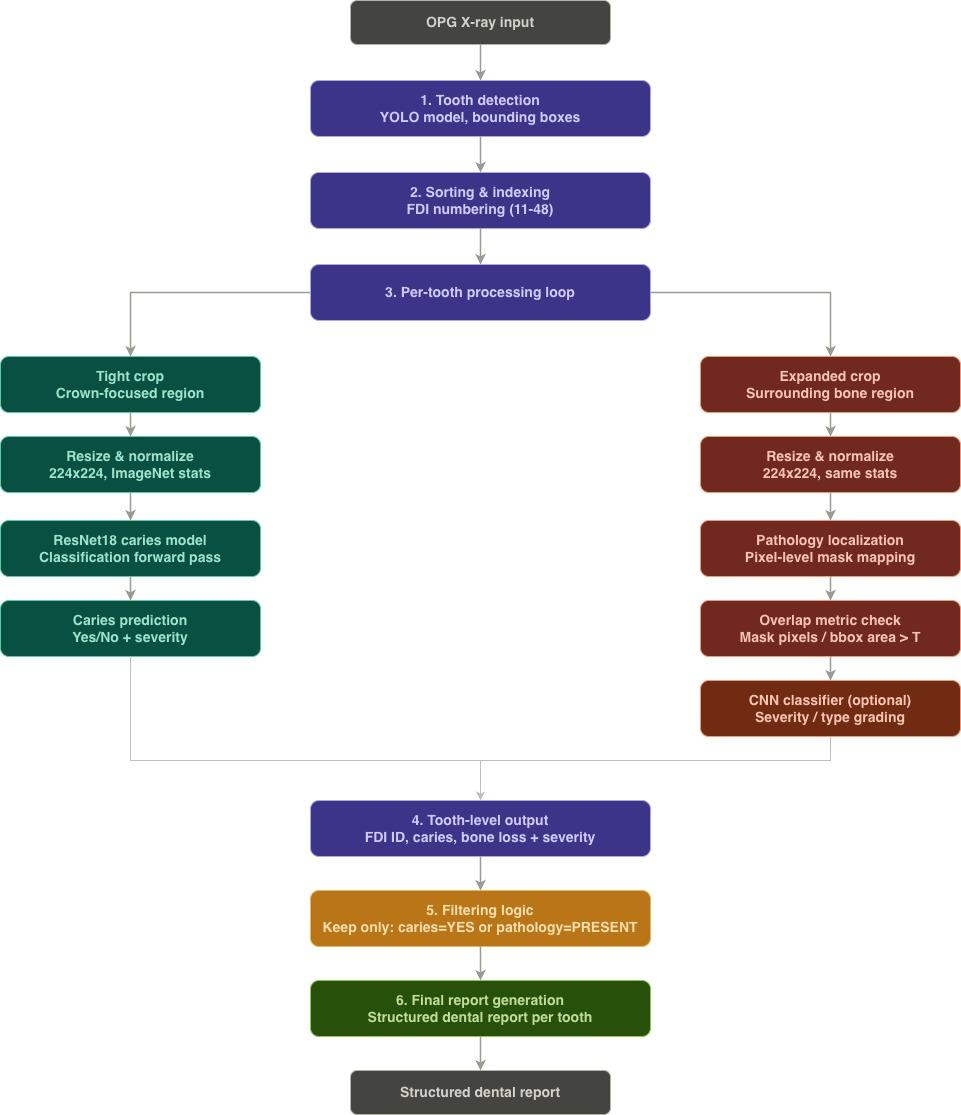
\includegraphics[width=0.62\textwidth]{figures/phase2/p2_3_01_target_pipeline.jpg}
\caption[Phase 2 target architecture]{The target end-to-end architecture drawn in the Phase 2 report
(Figure 3.1 there).}
\label{fig:p2target}
\end{figure}

\begin{table}[!htbp]
\centering
\caption[Phase 2 target design against the as-built design]{Phase 2 target design against the
as-built design, with the reason for each change.}
\label{tab:target-vs-built}
\small
\begin{tabularx}{\textwidth}{@{}L{3.0cm}L{3.6cm}L{3.8cm}Y@{}}
\toprule
Element & Phase 2 target & Phase 3 as built & Reason\\
\midrule
Numbering & Sort boxes into FDI order & Learned ResNet18 head plus Hungarian one-to-one assignment & Sorting fails when teeth are missing or tilted; a learned head with a one-to-one constraint cannot emit duplicate codes\\
Caries & Tight-crop classifier & Whole-image lesion detector, crop classifier retained & Five repairs of the classifier failed; the detector met a pre-registered rule\\
Bone loss & Overlap-labelled classifier with severity & Abnormality flag, severity withheld & The label marks expert abnormalities, not bone loss; the severity head did not beat a position prior\\
Filtering & Keep only positive teeth & Report every tooth, with an assessable flag & A missing tooth must be distinguishable from a healthy one\\
\bottomrule
\end{tabularx}
\end{table}

\section{Design Rationale}

The tooth-centric formulation was chosen over an image-level classifier because the deliverable is a
tooth-wise report, not one disease flag for the whole OPG. A modular pipeline is also the practical
answer to the available data: DENTEX provides tooth-level caries labels, Tufts is richer for
abnormality masks after region-to-tooth mapping, CariesXrays provides lesion boxes, and no single
dataset contains every label in one consistent format. A monolithic multi-task model would add
supervision mismatch without a clear advantage.

ResNet18 is the common backbone of the four classifier heads because it is light, well understood
and stable under transfer learning on small dental datasets; larger backbones were avoided because
the extra capacity raises overfitting risk without a demonstrated benefit. The two detectors are
YOLOv11l~\cite{jocher2024yolo11}, which balances accuracy and speed on a large panoramic image.

The modular design moves responsibility to integration: numbering, report assembly, consistency
checks and confidence handling must make independently trained models behave as one system. Phase 3
therefore added four mechanisms:
\begin{itemize}
\item a one-to-one assignment that forbids duplicate FDI codes;
\item an assessability rule that marks a tooth whose number is uncertain;
\item a check that refuses to fuse stage outputs of different lengths;
\item a limitations block in the report, keyed to the hash of each checkpoint that ran.
\end{itemize}

The caries stage changed form during Phase 3. The per-crop classifier of Phase 2 sees one tight crop
and answers yes or no, a task in which a strong positional prior can earn much of the score; five
direct repairs of it, each against a same-day control, gave no gain that separated from zero
(Section~\ref{sec:res-rq2}). The task was therefore changed to locating lesions on the whole image,
under an acceptance rule committed before any candidate was trained, and the classifier was kept as
a selectable alternative. % {C071}
